The purpose and ambition are to create a \CodeName extension build up on the core API explained in chapter \ref{chp:api}, to demonstrate the opportunities with a tangible and present example to set a standard. The extension seeks to model a data access layer (DAL) as a MapReduce framework (outlined in definition \ref{def:mapreduce}) for \CodeName like Hadoop for HDFS.

\section{Investigation}
The initial idea and thoughts were to create a bridge between the DAL of Disco (described in section \ref{sec:related}) and the API of \CodeName and thereby create a combined integration of the two systems, such that \CodeName would be an optimized and semantic-intelligent replacement for DDFS (Disco Distributed File System). The Disco end-user experience is written in Python programming language like \CodeName and thus would be more convenient to incorporate, rather than frameworks such as Hadoop, which is written in Java.
\newline

The first and foremost reason to design and implement an entirely new framework and thereby discard the Disco based solution was due to the demand and desire to have full control across the whole execution stack from the disk to the end-user input fields. A second and likewise significant reason is the optimization opportunities of having control of the full implementation such as caching of temporary and final results and data accessing.

\section{Assumption}
A small but sufficient number of assumptions has been put together, based on the brief but necessary investigation and the knowledge obtained by the examination of related work in section \ref{sec:related}, to limit the extension to the project scope:

\begin{itemize}
	\item The solution is targeted and used for big data analysis.	
	\item Data is assumed to be research and scientific related material. 
\end{itemize}
, which generally is inspired and based on the ones for \CodeNameShort, listed in section \ref{sec:assumption}.
\newline

Additionally, it is a requirement and thereby an assumption that the \texttt{OperationContext}s (defined in section \ref{sec:operation}) of the datasets can be modeled in terms of a MapReduce scheme.

\section{Objectives} \label{sec:bdae-objectives}
Based on the assumptions and the general knowledge taught by studying similar frameworks has following objectives been composed:
\begin{itemize}
	\item Utilize the \CodeName storage system and its API to create MapReduce based DAL.
	\item Define and design a collection structure to batch similar datasets.
	\item Implement predefined templates for common data structures to reduce redundant tasks for the end-users.
	\item Characterize a domain specific access model.
	\item Load complex data structures such as NetCDF\cite{PageNetCDF} or HDF5\cite{PageHDF5}\cite{Collette:2013:Python} in an intelligent and thus efficiently way to reduce I/O cost.
\end{itemize}

\section{Overview}
BDAE (\textit{/b'dei'/}) is the name and acronym of the big data analysis engine targeting MapReduce operations that are implemented. The solution is built solely using the \CodeName API as illustrated in figure \ref{fig:bdae-overview} and extending existing core components primarily from the foundation package, explained in chapter \ref{chp:components}.

\begin{figure}
	\centering
	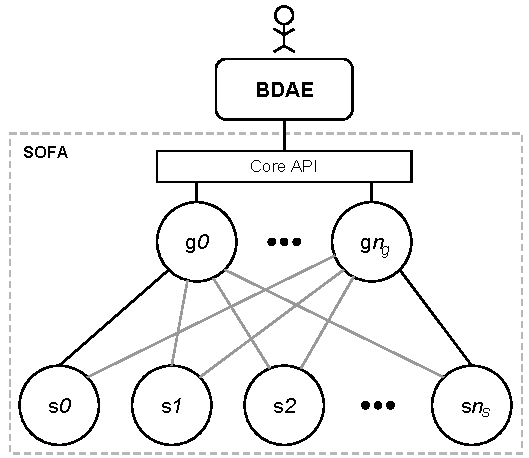
\includegraphics[scale=0.9]{pdf/bdae-overview.pdf}
	\caption[General overview of the BDAE]{General overview of the BDAE integration into \CodeName with same notation as in Figure \ref{fig:sofa-overview}. \label{fig:bdae-overview}}
\end{figure}	


\subsection{Dataset}
The \texttt{SofaBaseObject} defined in section \ref{sec:sofabaseobject} has been extended and delimited along with the requirement of the functions defined in the \texttt{OperationContex}, as a consequence of the chosen execution model. 
\begin{itemize}
	\item A \texttt{MapReduceDataset} has been defined which requires functions executed on the data to be ordered into a \texttt{map} and a \texttt{reduce} category. 
	\item All functions defined in an extended \texttt{OperationContex} is at runtime verified towards the two categories since the MapReduce execution model prescribes that each operation has at least one map function and at most one reduce function as the.
\end{itemize}

\section{Collection}
A dataset in \CodeName is defined by a dictionary with meta data and a list of associated semantic blocks, as previously mentioned in section \ref{sec:sofabaseobject}, but this meta data structure can with slightly modifications also be used as a descriptor for a collection of similar datasets, as was one of the objectives listed in section \ref{sec:bdae-objectives}:

\begin{quotation}
	\textit{"Define and design a collection structure to batch similar datasets."}
\end{quotation}

In other words; a collection in BDAE is defined as a marginally altered meta data dictionary with zero-length list of associated semantic blocks, that nevertheless obeys the interface of the \texttt{SofaBaseObject}, which is a required for any type of data in \CodeName.

\section{MapReduce}

\section{User tiers}
\subsection{Data scientist}
\subsection{Data manager}
\subsection{System administrator}

\section{Templates}
\subsection{Module binder}
\subsection{Text}
\subsection{Image}
\subsection{Numpy Array}
\subsection{NetCDF}

\section{Libraries}
\subsection{\texttt{libbdaescientist}}
\subsection{\texttt{libbdaemanager}}
\subsection{\texttt{libbdaeadmin}}
\subsection{Web}
\subsection{Android App} \label{sec:bdaeapp}